
In the following, we will summarise the results obtained for the IRTF
data set. We deal with the different physical paramenters in separate
Sections. We start by reporting the cross validation Root Mean Square
Errors (RMSE) for the five-fold cross-validation strategy, and
subsequently discuss the accuracy of the predictions with respect to
literature values where available.

\subsection{Effective temperature models}

Table \ref{tab:model_TSD} summarises the RMSE for the complete set of
models: the minimum $\chi^2$ estimate based on the full spectrum
($\chi^2$), the projection pursuit regression based on the ICA
components (PPR-ICA) and some models trained on the spectral
features proposed by the GA (GA-RF, 
GA-GBM, GA-SVR, GA-NNET, GA-MARS, GA-KPLS). For each model, we report
the RMSE obtained for several noise levels of the training sets. 
We use the following notation: RMSE represents the RMSE
obtained for a model trained and tested on BT Settl spectra. 
SNR=$\infty$ corresponds to noiseless spectra. 
The RMDSE means the root median square error, as a way to provide 
robust estimation against outliers.

\newcommand{\ra}[1]{\renewcommand{\arraystretch}{#1}}
\begin{table*}\centering
\ra{1.3}
\begin{tabular}{@{}rrrcrrcrr@{}}\toprule
& \multicolumn{2}{c}{$SNR = 10$} & \phantom{ab}& \multicolumn{2}{c}{$SNR = 50$} &
\phantom{ab} & \multicolumn{2}{c}{$SNR = \infty$}\\
\cmidrule{2-3} \cmidrule{5-6} \cmidrule{8-9}
$Regression Models$ & $RMSE$ & $RMDSE$ && $RMSE$ & $RMDSE$ && $RMSE$ & $RMDSE$ \\ \midrule
$\chi^2 BTSettl$    &  232.55 & 100.00 && 235.25 & 120.00 && 232.45 & 100.00 \\
$ ICA+ ppr$         & 241.93 & 127.75 && 241.83 & \bf{99.14} && 279.70 & 161.90 \\
$rf $               & 308.46 & 183.03 && 247.65 & 136.48 && \bf{167.21} & 135.23 \\
$ gbm $              & 287.21 & 159.92 && 247.93 & 149.01 && 233.22 & 112.59 \\
$ svr $         & \bf{221.46} & 122.36 && 281.21 & 150.59 && 299.05 & 160.22 \\
$ nnet $            & 283.44 & 191.58 && 264.16 & \bf{114.35} && 326.35 & 211.81 \\
$ knn $             & 238.18 & 120.00 && \bf{232.36} & 137.50 && \bf{219.14} & \bf{100.00}  \\
$ mars+ bagging $   & 253.14 & 113.47 && 254.00 & \bf{95.44} && \bf{226.14} & 133.49 \\
$ kpls $            & 275.48 & 120.00 && 299.88 & \bf{118.61} && 387.06 & 217.53 \\



% \begin{table}
% \begin{center}
% \begin{tabular}{rrrrrrrrrrrr}
% \begin{tabular}{rrrr}

% \hline
% Regression Technique & SNR=10 & SNR=50  & SNR=\infty \\ 
%  SNR & $\chi^2$ & PPR-ICA & C-??? & GA-RF & GA-GBM & GA-SVM & GA-NNET & GA-KNN & GA-MARS & GA-KPLS & GA-RULE \\
%\hline
%$\chi^2$ & 
%ICA+PPR  &

%CV-RMSE$\infty$ &        &        &  & 232.10 & 233.22 & 299.05 & 326.35 & 219.14 & 226.14 & 387.06 & 332.92\\
%CV-RMSE10 & 232.55 & 241.93 &  & 308.46 & 287.21 & 221.46 & 283.44 & 238.18 & 253.14 & 275.48 & 260.76\\
%CV-RMSE50 & 235.25 & 241.83 &  & 247.65 & 247.93 & 281.21 & 264.16 & 232.36 & 254.00 & 299.88 & 270.09\\
%LI-RMSE$\infty$ &  &  &  &  &  &  &  &  &  &  & \\
%LI-RMSE10 &  &  &  &  &  &  &  &  &  &  & \\
%LI-RMSE50 &  &  &  &  &  &  &  &  &  &  & \\

%\hline
\bottomrule
\end{tabular}
\caption {RMSE and RMDSE for the various regression models that predict $T_{eff}$ (K).} 
\label{tab:model_TSD} 
% \end{center}
\end{table*}

%Table \ref{tab:model_TSD} shows that the performance of classifiers
%based on the full spectrum (or in a compressed version in the form of
%ICA components) and on features derived from limited spectral bands is
%equivalent. The difference between the performances of best classifier
%(GA-KNN; best on average over SNR), the minimum $\chi^2$ classifier,
%and the PPR-ICA classifiers are not statistically significant. We
%interpret these small differences as an indication that there is as
%much information spread over the entire spectrum shape as can be
%distilled from a few spectral bands. In any case, it is evident that
%the RMSE is significantly above the grid spacing in temperature ({\bf
%I think this is 100K but it depends on the answer to my questions
%whether the interpolated grid was used or not.})

The comparison with the effective temperatures compiled
by \cite{cesetti} does not show significant differences either. In
general, all classifiers tend to predict lower effective temperatures
than those in the literature.

\begin{table*}\centering
\ra{1.3}
\begin{tabular}{@{}lrrr@{}}\toprule
& {$SNR = 10$} & {$SNR = 50$} & {$SNR = \infty$}\\ \midrule
$\chi^2 $    &  -77.45 & -86.88 & -85.00 \\
$Rule Regression$ & -101.78 & -38.38 & 169.74 \\
$rf $ & -172.61 & -127.12 & -5.32 \\
$gbm $ & -140.87 & -108.53 & 31.70 \\
$svr $ & -57.62 & -2.93 & 91.68 \\
$nnet$ & -146.57 & -36.12 & 39.10 \\
$knn $ & -75.57 & -109.85 & -66.60 \\
$mars + bagging $& -56.96 & -87.88 & 98.22 \\
$pls $ & -120.32 & -4.23 & 213.68 \\

\bottomrule
\end{tabular}
\caption {Bias for $T_{eff}$ (K) over the Cesseti estimation.} 
\label{tab:model_Tbias} 
% \end{center}
\end{table*}


Most models show remarkably similar distributions of the
predictions when trained with different SNR levels. In the cases of
GA-MARS, GA-KNN, and GA-SVR this is the case even in the unrealistic
scenario of SNR=$\infty$.

In general, models tends to produce better behaved solutions (with
smaller biases and less scatter) for SNR=50. We interpret this value
as representative of the SNR of the majority of spectra in the IRTF
collection. We have found in previous studies that, at least for input
spaces constructed from ICA compressions of the spectra, it is not
necessary to adapt the training set SNR to match exactly that of the
prediction set. On the contrary, we find that two regimes are
sufficient to obtain proper results. The two regimes are separated at
SNR=10. The model trained with SNR=50 spectra gives close to optimal
results for spectra with SNRs above 10, while below that limit the
same situation applies holds for the model trained with SNR=10
spectra. {\bf I should move this explanation to the beginning of the
section or to the methodology section.}




%\begin{table}
%\begin{center}
%\begin{tabular}{rrrrrrr}
%  \hline
%  SNR & Features & SVM & RF & GAM  & MARS  \\
%  \hline
%  \multirow{2}{*}{50}  &  Cesetti et al. & 81.6 &  83.3 & 163.5 & 91.9 \\
%      &  GA             & 91.4 & 82.2 & 161.1  & 91.9  \\
%  \multirow{2}{*}{10}  &  Cesetti et al. & 135.8 & 138.5 & 268.8 & 166.8  \\
%      &  GA             & 123.2 & 122.6 & 212.6 & 130.9  \\
%   \hline
%\end{tabular}
%\caption { RSME for different models predicting $T_{eff}$ [K].} 
%\label{tab:model_TSD} 
%\end{center}
%\end{table}

%After calculating the bartlett test for both cases of SNR it was 
%seen that variances are homogeneous since p > 0.05, and 
%the Flinger-Killen shows that homokedascity is verified, 
%then F-ANOVA test makes clear that there is no significative 
%difference between models. Then, it is possible to conclude
%that quality of features from both sources are equivalent
%regarding modeling capability, even when GA only has proposed five
%features and Cesetti et al. requires seven features.

%As an alternative to build modles based on bandpasses, 
%a similiar methodology to the one depicted in (\cite{2013A&A...550A.120S})
%was implemented.

%For the projection an Independend Component Analysis (ICA) with ten dimensions
%was used and for Temperature regression an optimized SVM 
%with parameters of C=10 and $\epsilon$=0.001.

%Considering the Gravity case, the most suitable ICA had twentysix dimensions and the 
%best SVM parameters were C=1000 and $\epsilon = 0.001 $. This was the same case
%for Metallicity.

%In terms of interpretation, this methodology looks to predict the physical paramenters
%by considering the whole star spectrum instead of information provided 
%by specific bands. Thus it can be interesting to analyze suitability 
%for prediction against the other approach.

%In the same sense it was decided to consider direct selection, which is
%also a technique based on the whole espectrum but, instead of regressing
%specific parameters, the closest labeled spectrum to the one 
%under analysis is identified by a $\chi^2$ distance.
%This becomes possible as interpolation between labeled spectra can be
%easily performed.

We then compare the predicted effective temperatures with the spectral
types listed in the IRTF spectral library. We attempted a direct
comparison with the literature values gathered in \cite{cesetti} but
it only returns 57 
estimates of effective temperature for M stars. We converted the
spectral types into effective temperatures using the calibration
of \cite{2009ApJ...702..154S}.

{\bf TODO: Luis, cambiar spectral libraries por stellar atmosphere
models o synthetic spectral libraries}.

Forecast quality of models was tested by the error against the
temperature estimated based on the Spectral Subtype for each of the
IRTF available spectra (see \ref{ssub:TLSB}).  Both Root Mean Squared
Error (RMSE) and Mean Absolute Error (MAE) where calculated and it is
presented in the table~\ref{tab:model_Tvar}.

From this comparison several things arise:
\begin{itemize}
 \item {The behavior of $\chi^2$ distance is quite stable against SNR 
	in the original dataset (BT\_Settl) with a slightly better global 
	performace in fovour of SNR=50.}
 \item {Models trained with different SNR=$\infty$ have similar performance but heavy 
	differences appear when SNR features are considered.}
 \item {When synchronous behavior is observed FT00, FT11, FT55, the better SNR is 10.}
 \item {Best set of features to be used for forecast are those from SNR=$\infty$ (FT0b).}
 \item {As a conclusion the better performance was produced by FT01, followed by the FT51.}
\end{itemize}

In Figures~\ref{fig:comp01}~\ref{fig:comp02} the relationship between Temperature
estimated from the GA technique proposed features and modeled with different 
technqiues and the $chi^2$ with SNR=50 against the 
estimations provided by \cite{cesetti} can be seen.

\begin {figure}
 \centering
 \begin{subfigure}{.85\textwidth}
  \centering
  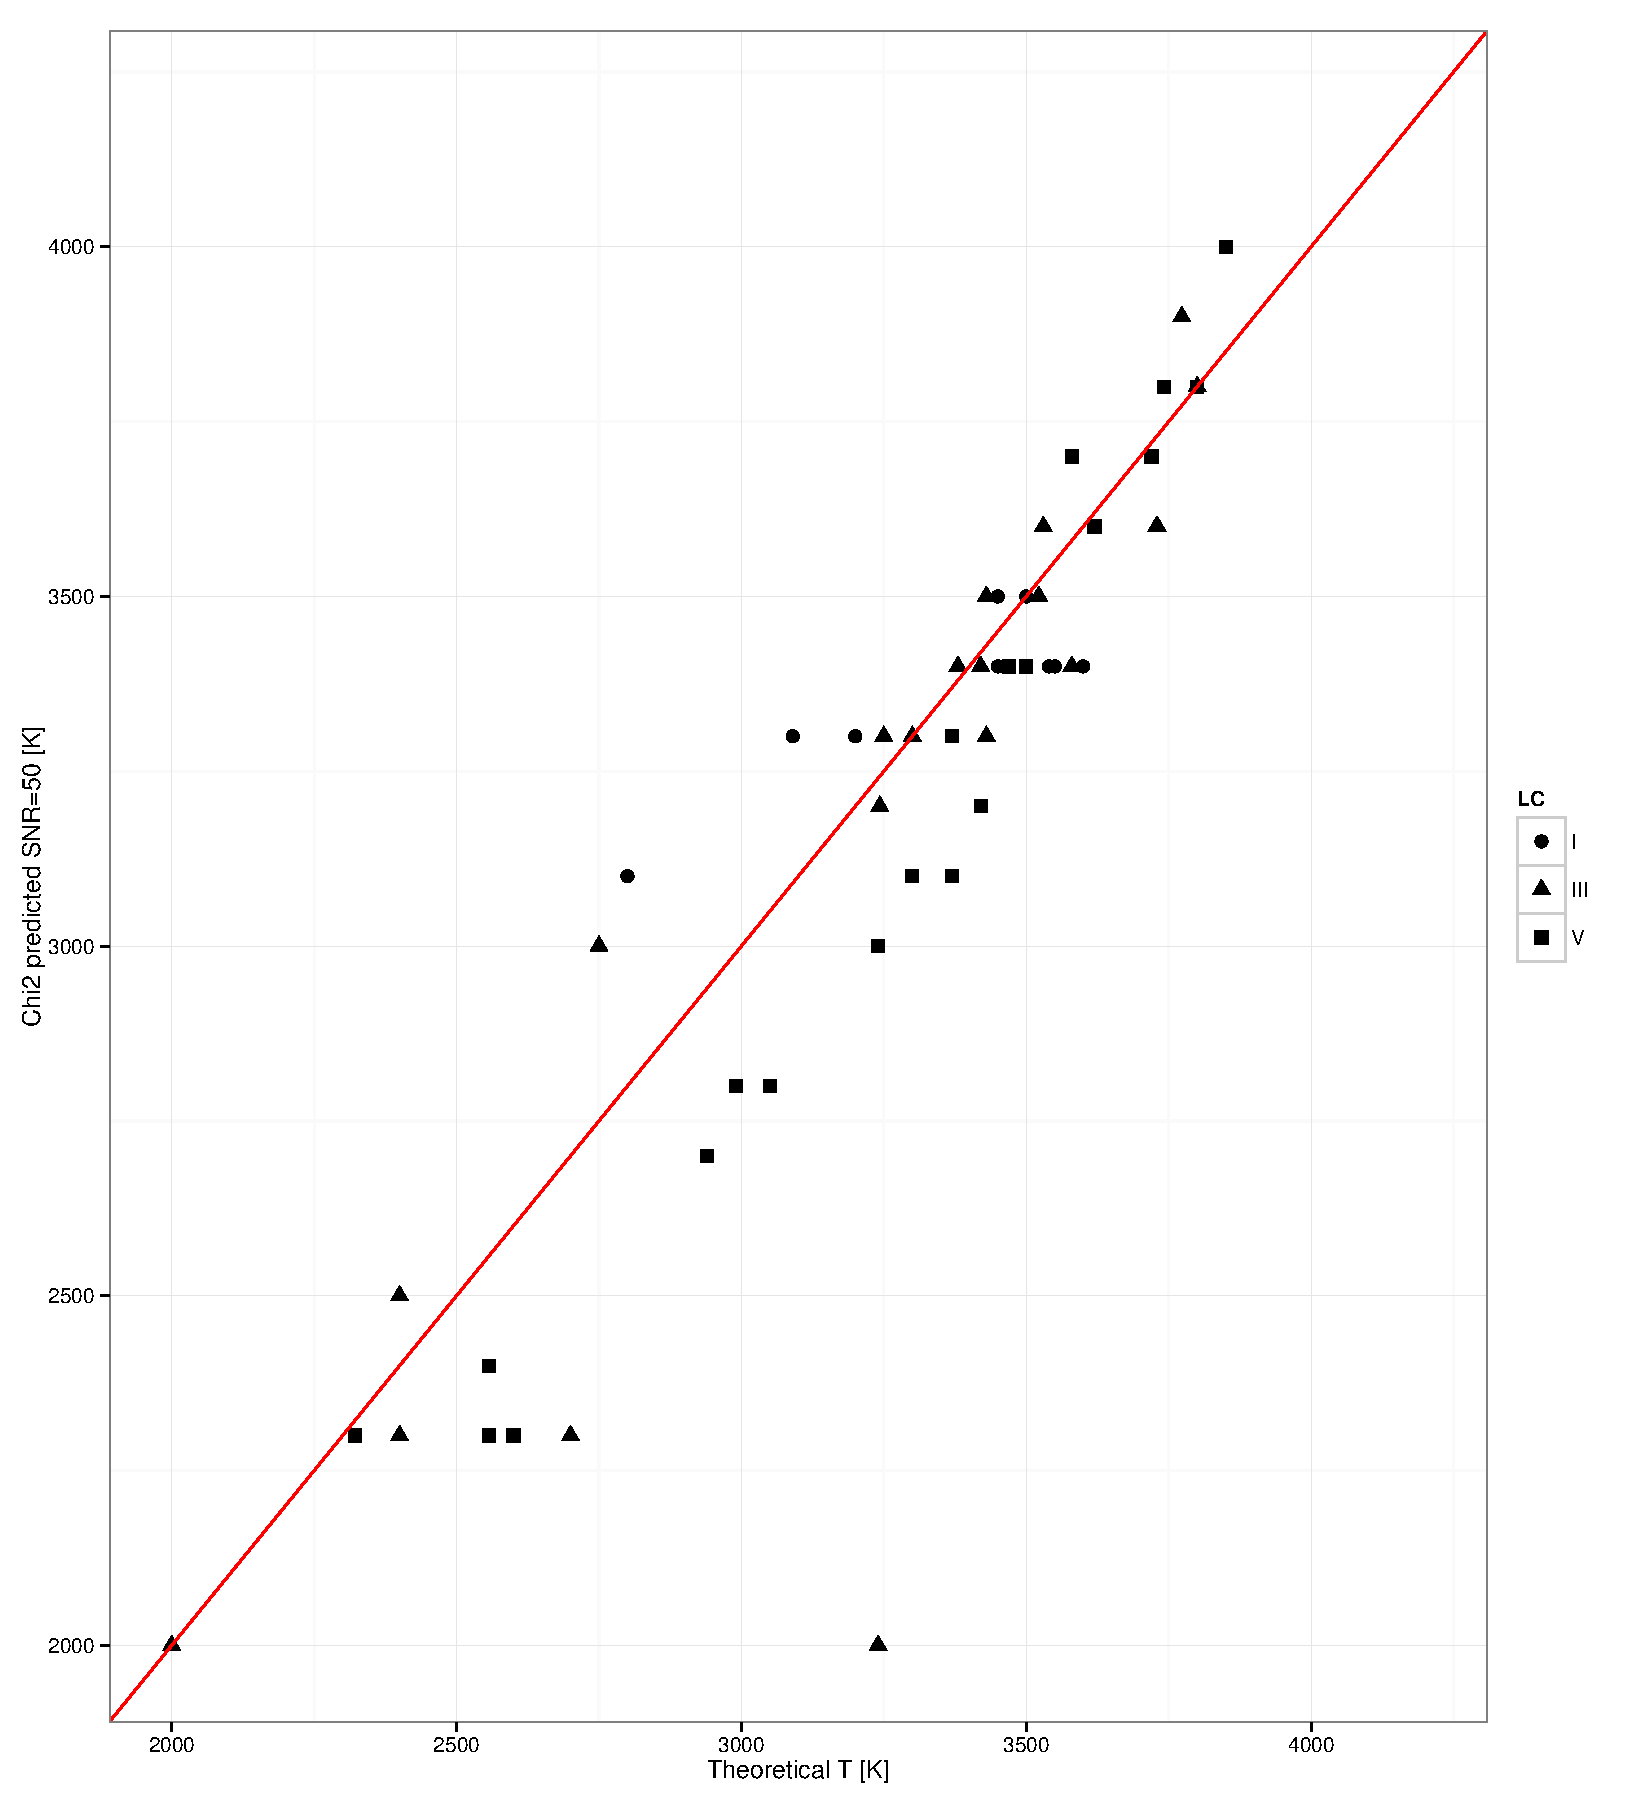
\includegraphics[width=11cm]{figs/irtf_T_chi250_Cesetti.pdf}
  \caption{Comparison between Temperature estimations from Cesetti 
  in x axis and the closest BT\_Settl spectra by $\chi^2$ at SNR=$50$ on y-axis}
 \label{fig:chi2_50_spt}
 \end{subfigure}
  \begin{subfigure}{.85\textwidth}
  \centering
  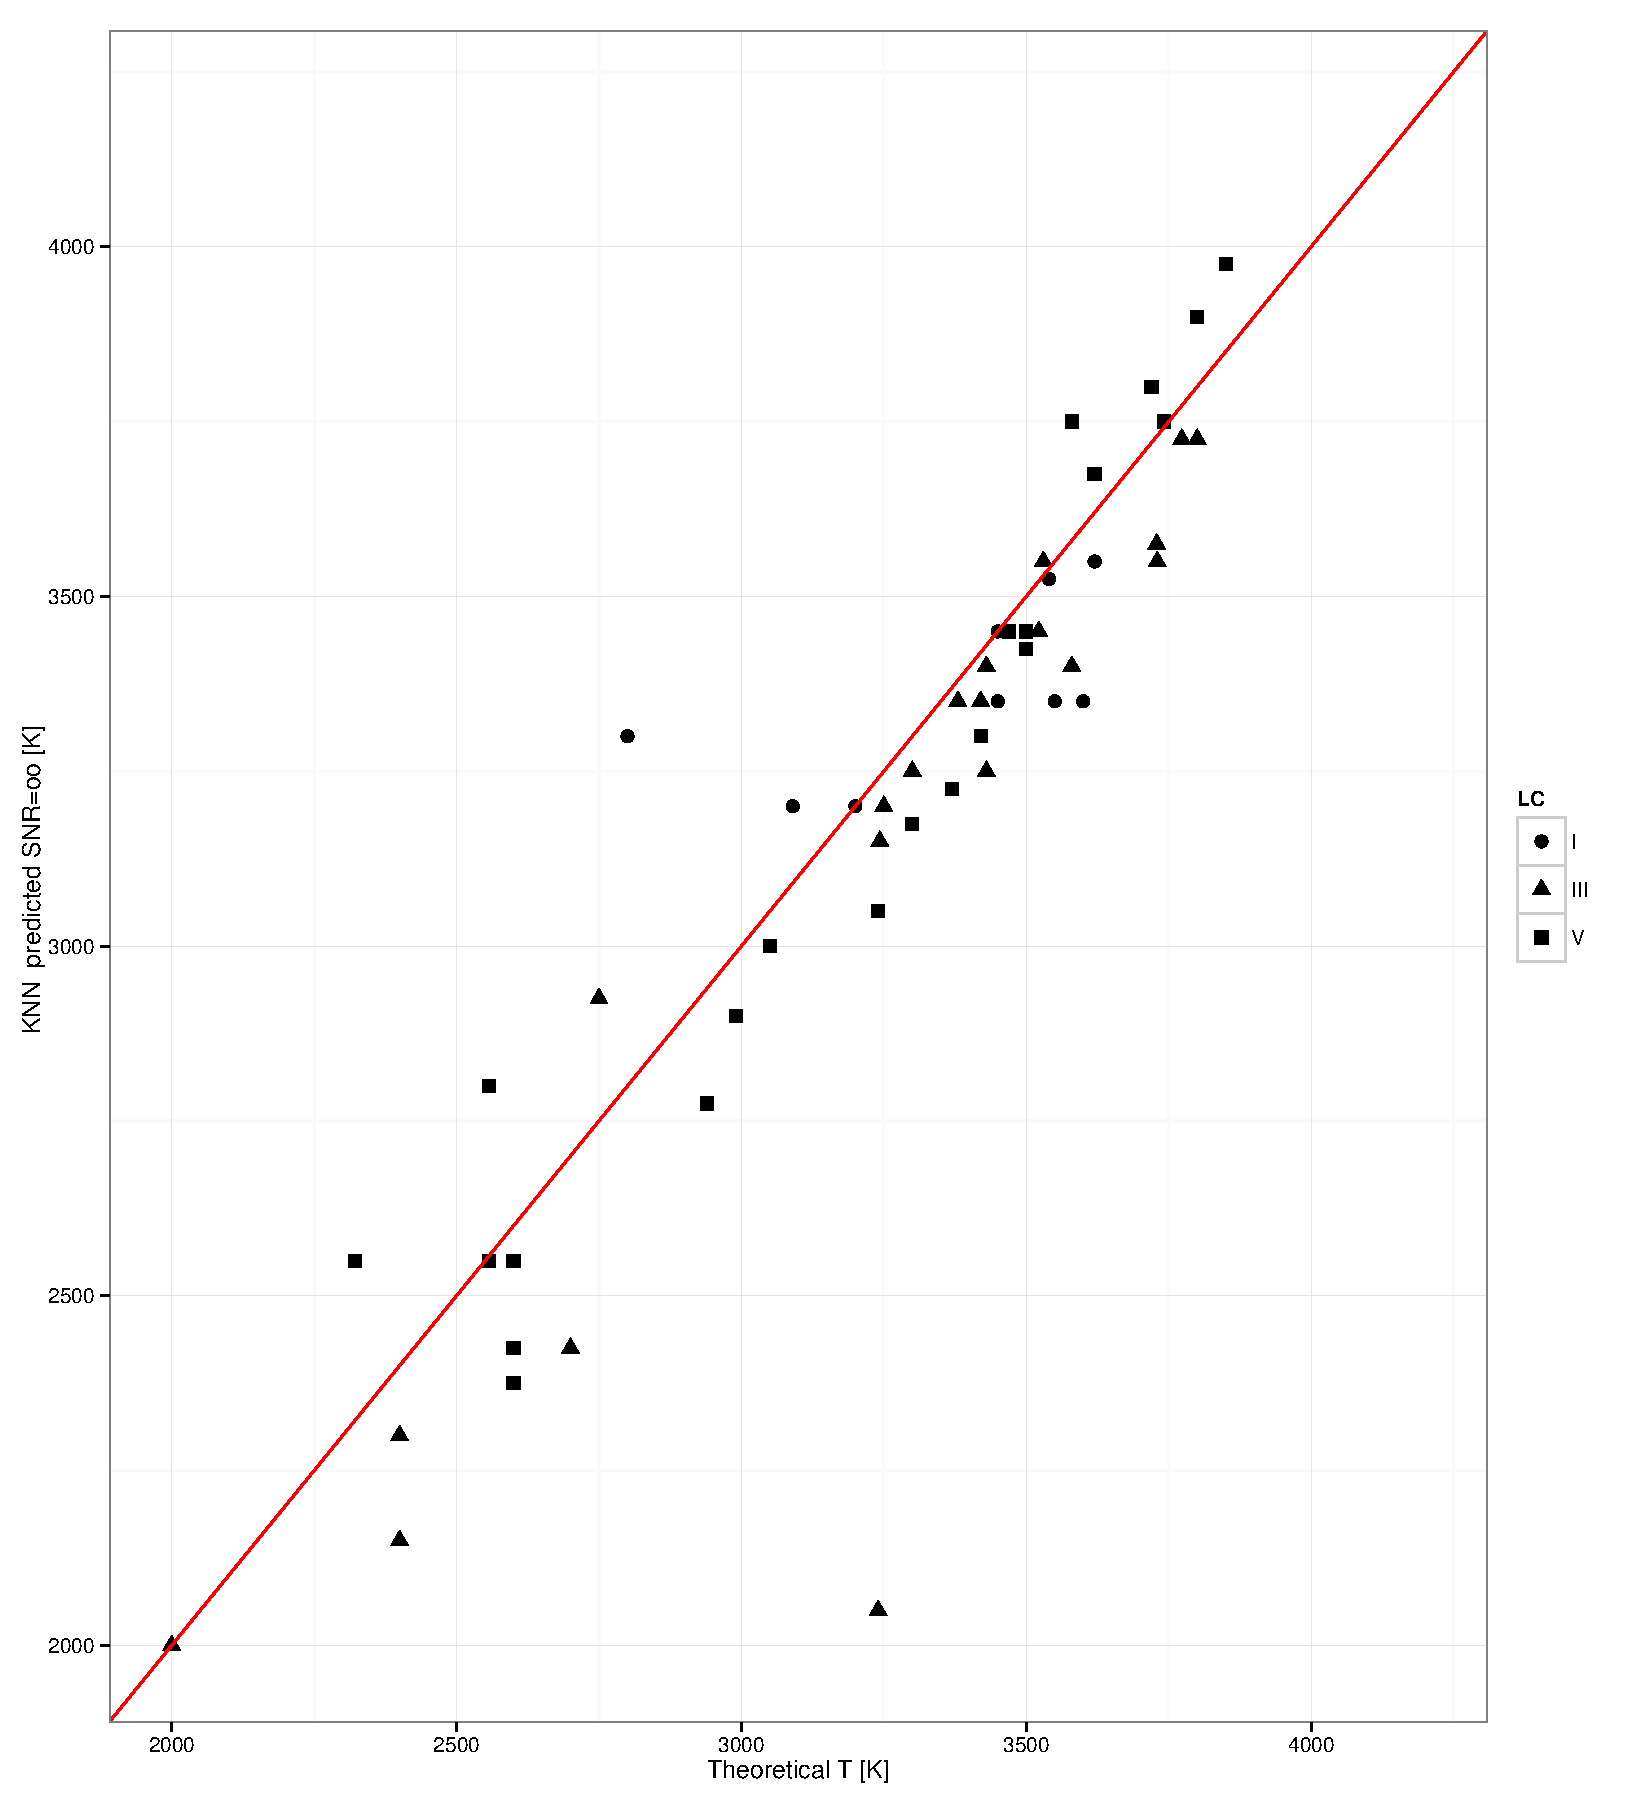
\includegraphics[width=11cm]{figs/irtf_T_knnoo_Cesetti.pdf}
  \caption{Comparison between Temperature estimations from Cesetti 
 in x axis and the KNN model for GA based features 
 at SNR=$\infty$ on y-axis}
 \label{fig:ga_too50ga_spt}
 \end{subfigure}
 \label {fig:comp01}
 \caption{Performance comparison between the $\chi^2$ based selection 
          and the band oriented features}
\end {figure}
 
 
\begin {figure}
 \centering 
 \begin{subfigure}{.85\textwidth}
  \centering
  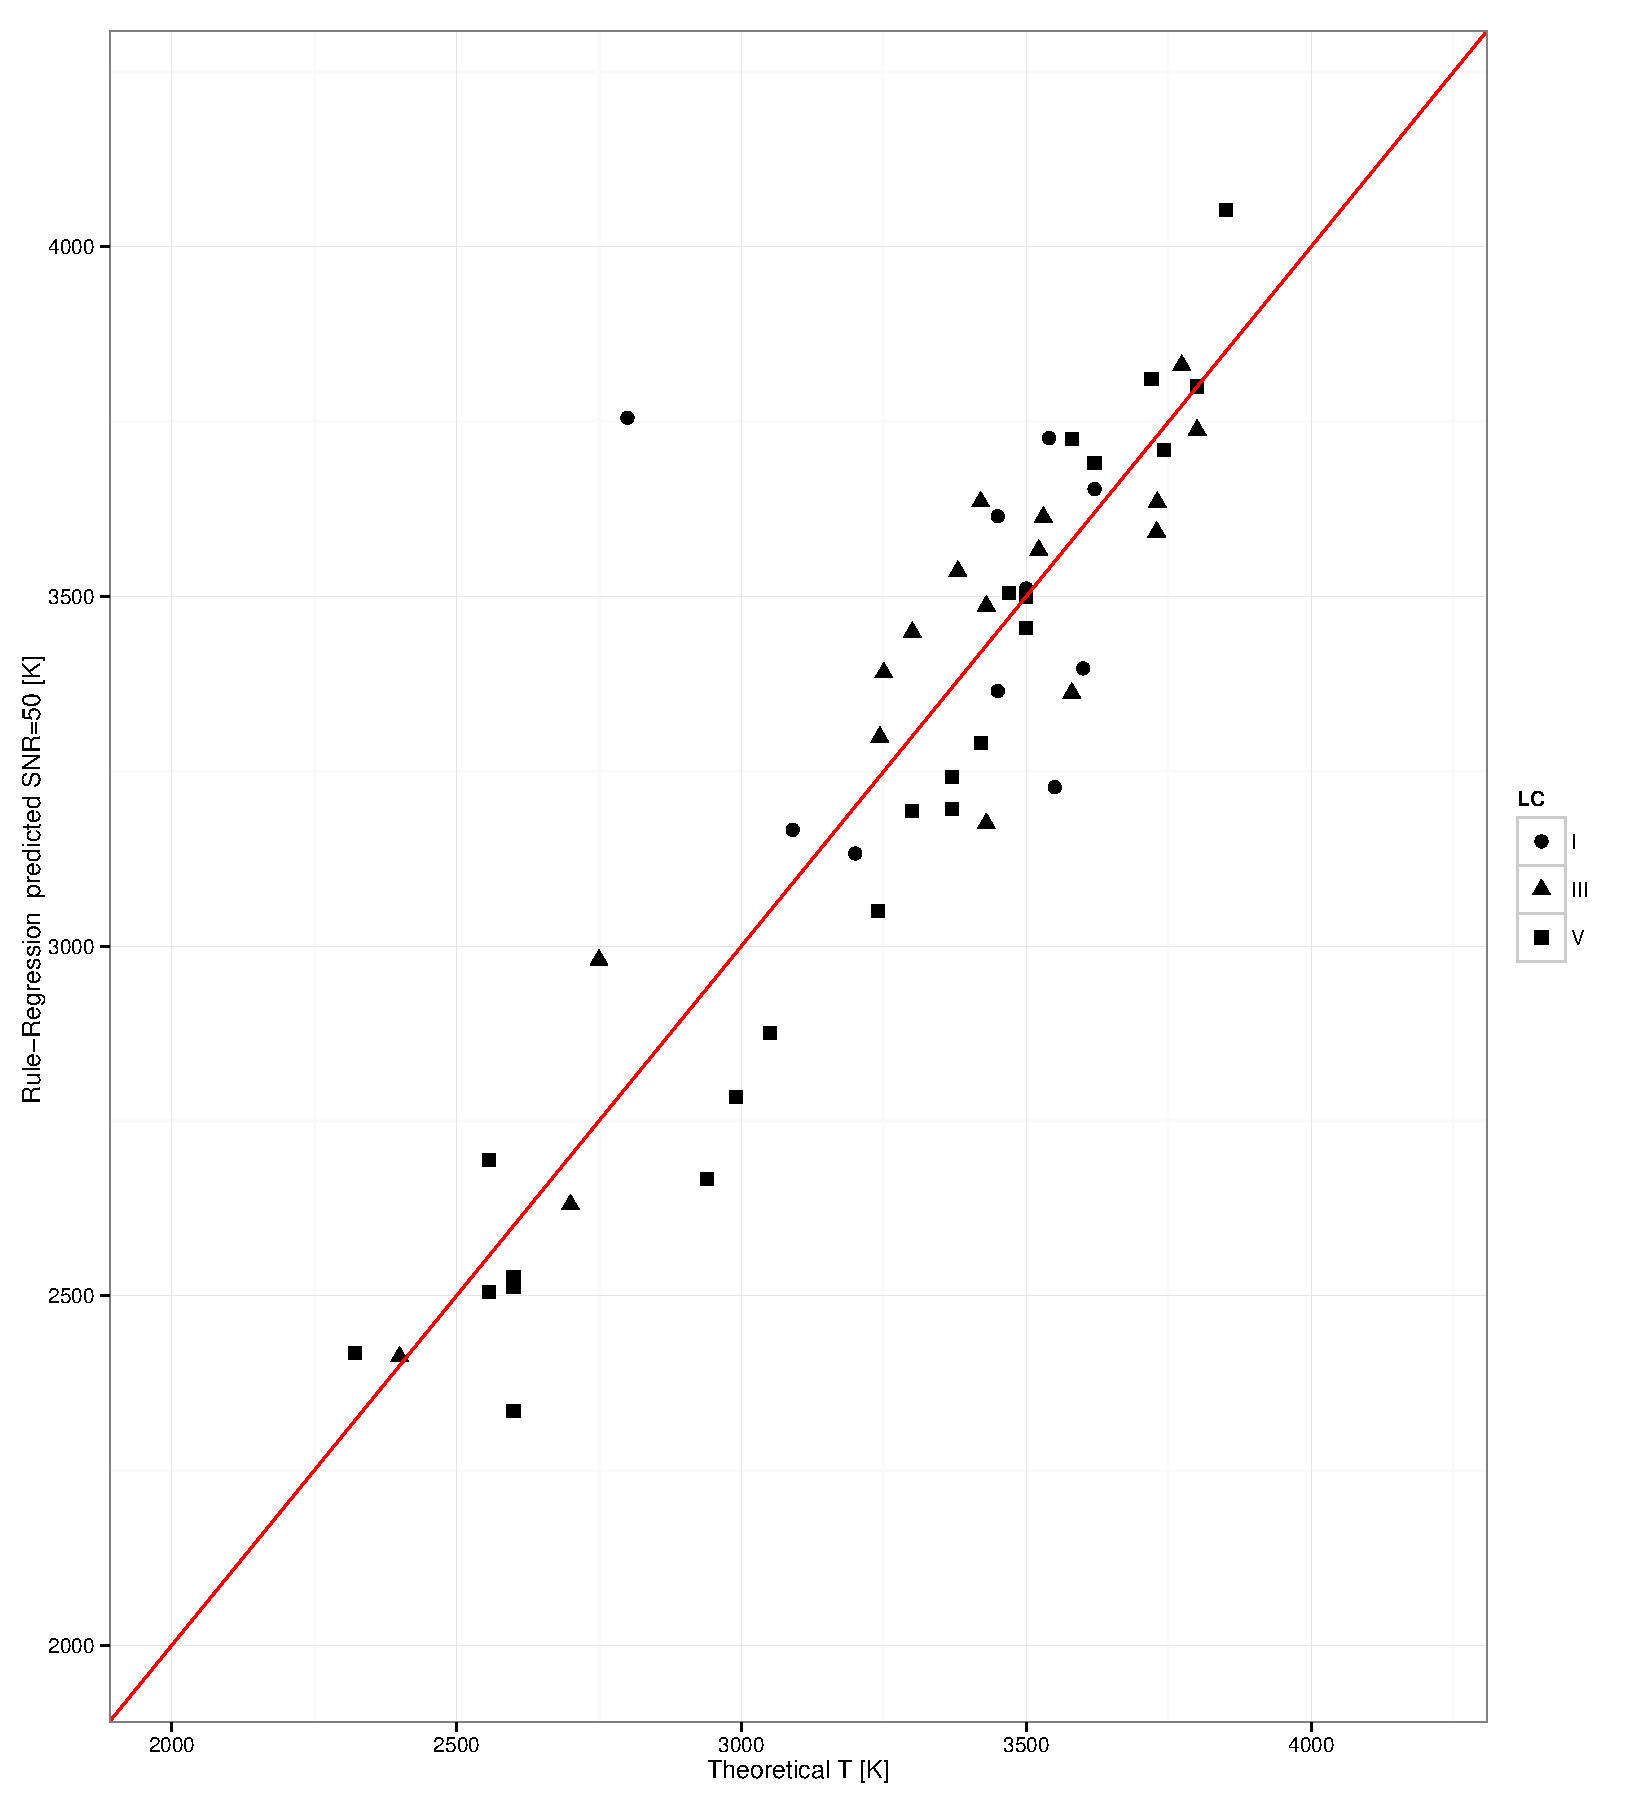
\includegraphics[width=11cm]{figs/irtf_T_rregoo_Cesetti.pdf}
  \caption{Comparison between Temperature estimations from Cesetti 
 in x axis and the Rule Regression model for GA based features 
 at SNR=$\infty$ on y-axis}
 \label{fig:ga_rr00ga_spt}
 \end{subfigure}
\begin{subfigure}{.85\textwidth}
  \centering
  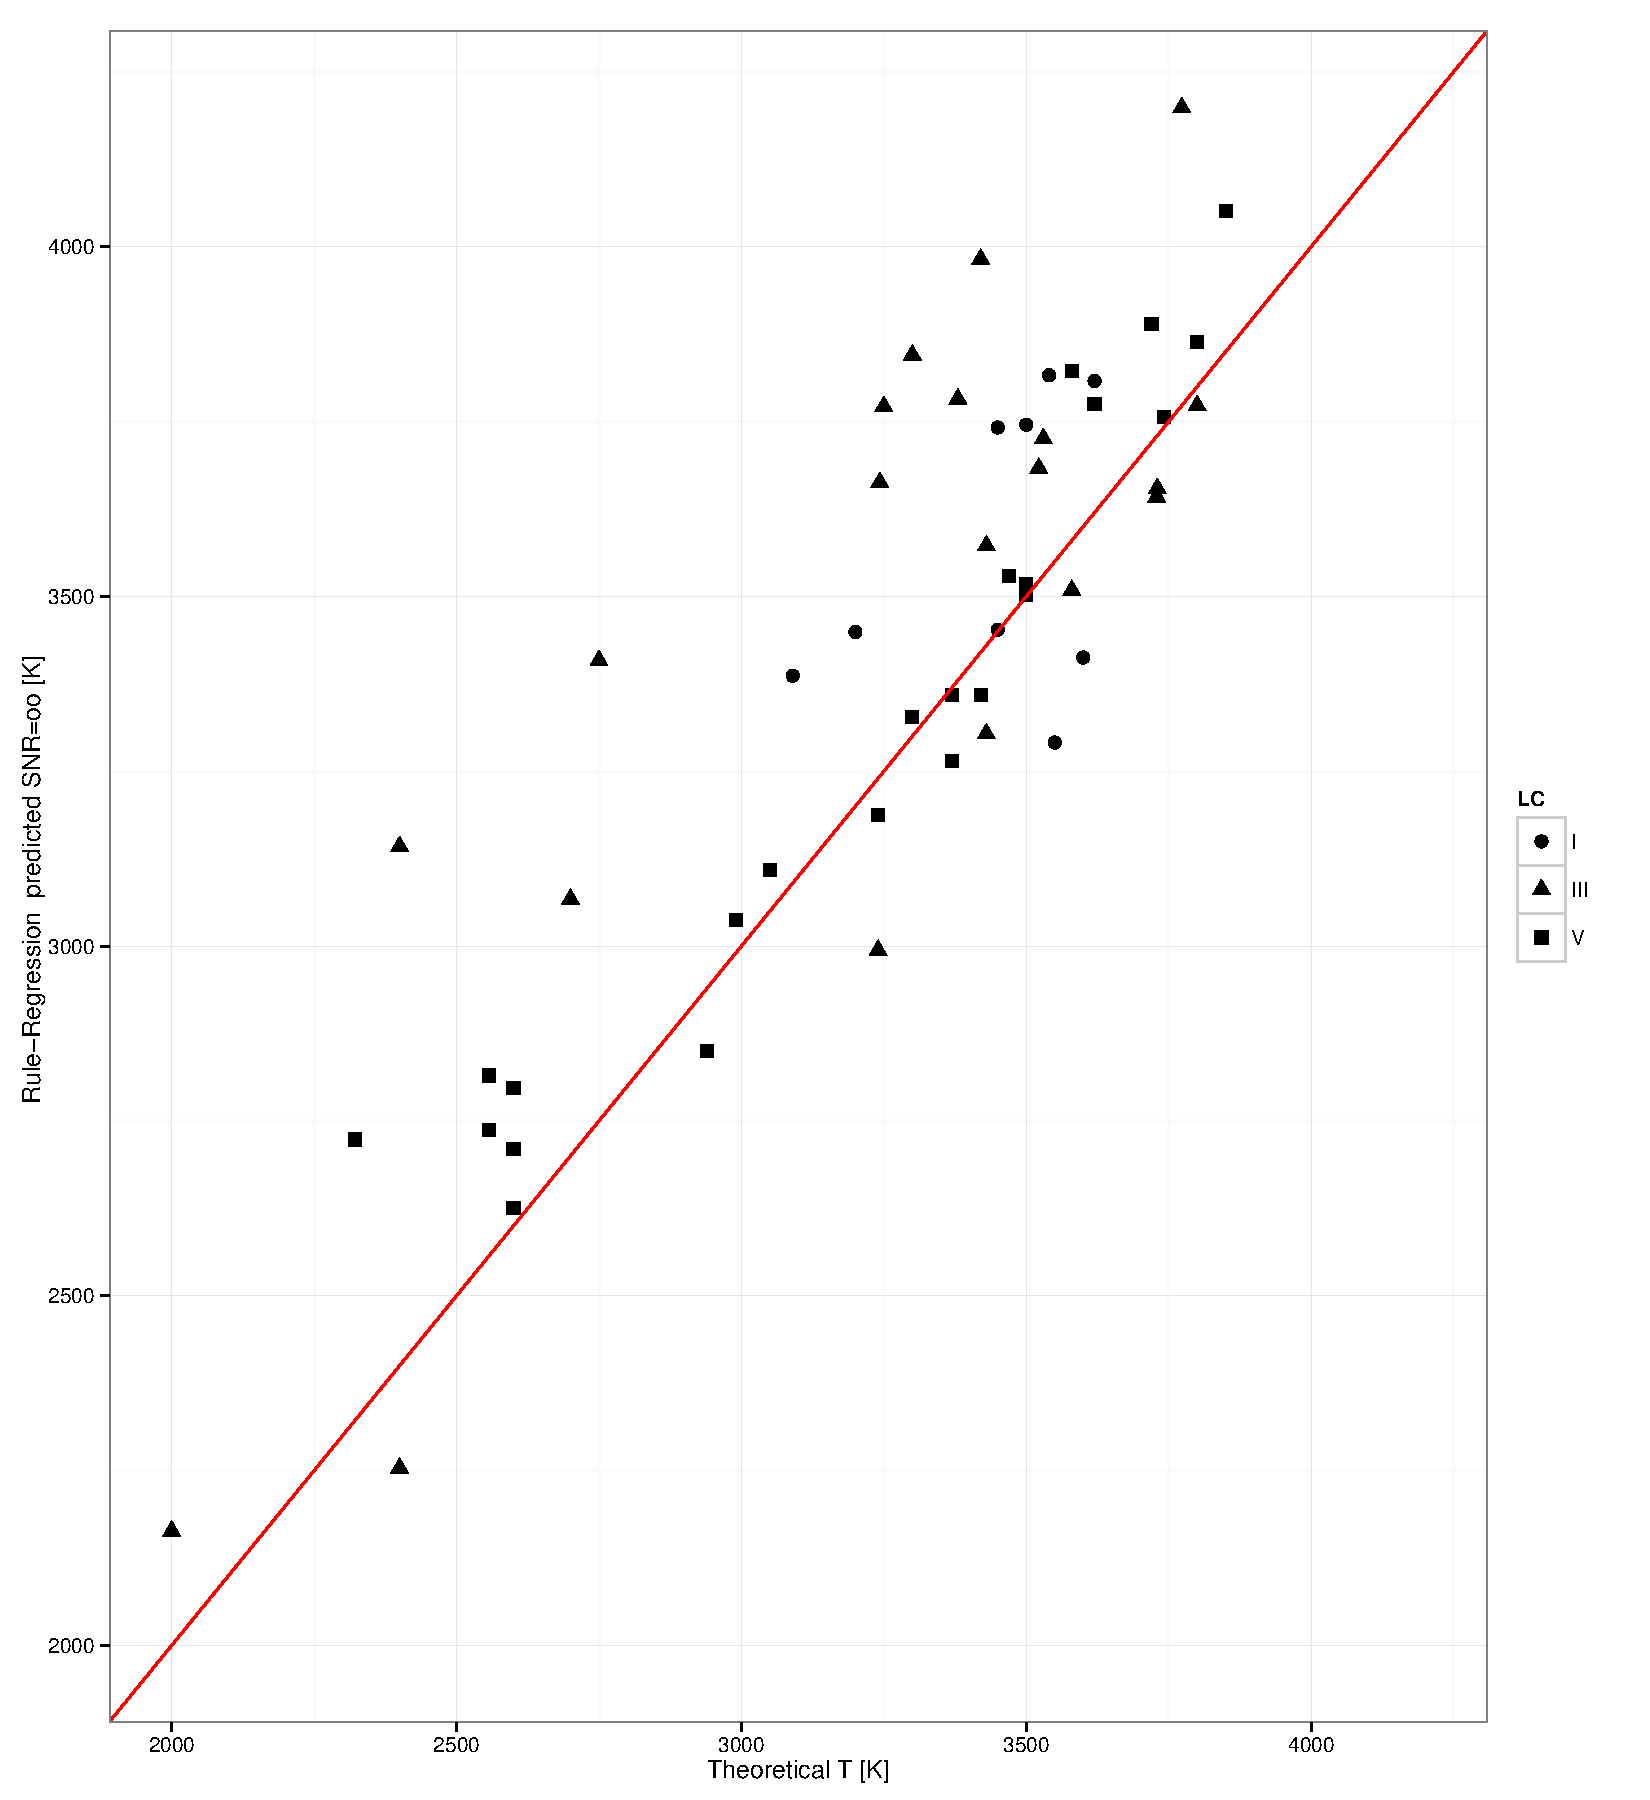
\includegraphics[width=11cm]{figs/irtf_T_rreg50_Cesetti.pdf}
  \caption{Comparison between Temperature estimations from Cesetti 
 in x axis and the Rule Regression model for GA based features 
 at SNR=$50$ on y-axis}
 \label{fig:ga_rr50ga_spt}
 \end{subfigure} 
 \label {fig:comp02}
 \caption{Performance comparison between two Rule regression based models with different SNR}
\end {figure}
%
% No le añado más discusión porque habría que interpretar algunas estrellas.
%

% En kile ^D Comenta y ^MayD descomenta
%
% Similarly Figure~\ref{fig:t10ga_tsb} shows the relationship against GA features 
% and Random Forest model trained by BT-Settl at SNR=10.
% 
% \begin {figure}
%  \begin{center}
%  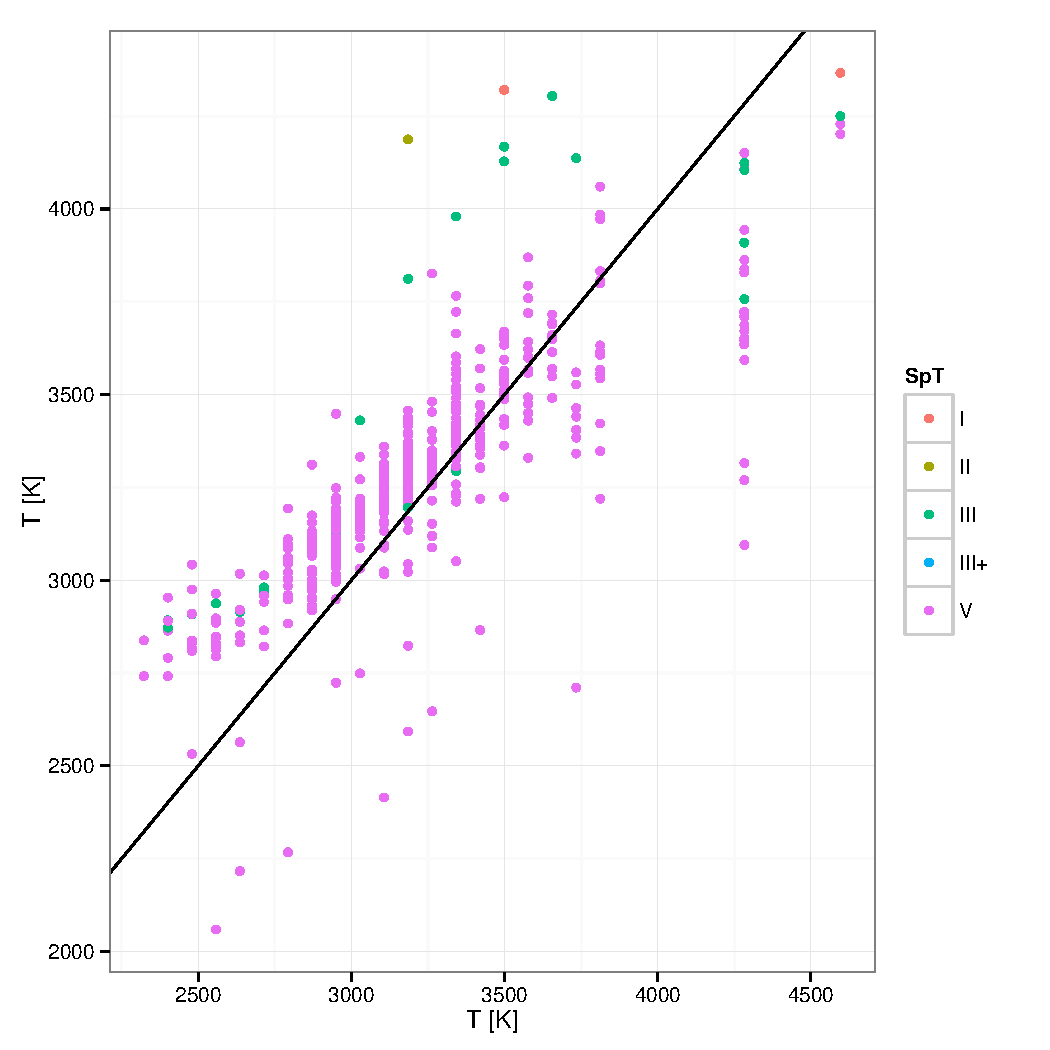
\includegraphics[width=6cm]{figs/T10GA_TSB.pdf}
%  \caption{Comparison between Temperature estimations from Spectral Subtype 
%  in x axis and the Random Forest for Ga based features trained with BT-Settl 
%  at SNR=10 on y-axis}
%  \label{fig:t10ga_tsb}
%  \end{center}
% \end {figure}


% No le añado más discusión de momento, hasta ver si tiene sentido poer toda esta
% fila de gráficas o es mejor producir algo más condensado.
%

\subsection{Surface gravity models}

The same approach can become useful to produce $log(G)$ estimations. 
Here comparisons can only be possible between GA based features, the 
global spectra based approach with $\chi^2$ distance
to be minimized and those stars with gravity was 
estimated in  \cite{2013A&A...549A.129C}.

The only difference with the methodology presented above is because
Temperature has been considered a fixed feature in the estimation of 
Gravity.

In Table~\ref{tab:models_G_rmse} 
we can see the analysis of performance between
the $\chi^2$ identificacion and the one based on features from the spectrum
depending on several classes of features. All of them have been carried out
against the \cite{Cesetti} estimations but, unfortunatelly those authors 
do not provide excessive number of IRTF class M stars to validate (just eight items).

%
% Gravedad teórica desde Cesseti para las IRTF
%
\ra{1.3}
\begin{table*}\centering
\begin{tabular}{@{}rrrcrrcrr@{}}\toprule
& \multicolumn{2}{c}{$SNR = 10$} & \phantom{ab}& \multicolumn{2}{c}{$SNR = 50$} &
\phantom{ab} & \multicolumn{2}{c}{$SNR = \infty$}\\
\cmidrule{2-3} \cmidrule{5-6} \cmidrule{8-9}
$Regression Models$ & $RMSE$ & $RMDSE$ && $RMSE$ & $RMDSE$     && $RMSE$       & $RMDSE$ \\ \midrule
$\chi^2 BTSettl$    &  0.82 & 0.45        && 0.93   & 0.61     && 3.5          & 3.48 \\
$ ICA+ ppr$         & \bf{0.54} & 0.48     && 0.34  & \bf{0.17} && \bf{0.72}   & \bf{0.57} \\
$rf $               & \bf{0.64} & \bf{0.38} && \bf{0.77} & 0.72    && \bf{0.53} & \bf{0.39} \\
$gbm $              & \bf{0.48} & 0.45    && \bf{0.61}  & \bf{0.47} && \bf{0.49} & \bf{0.41} \\
$ svr $             & \bf{0.66} & \bf{0.40} && \bf{0.63} & \bf{0.58}  && \bf{0.46}  & \bf{0.21} \\
$ nnet $            & \bf{0.78} & 0.61  && \bf{0.47} & \bf{0.44} && 1.2    & 0.97 \\
$ mars+ bagging $   & 0.84      & 0.57      && \bf{0.54} & \bf{0.37} && 0.99    & 0.76 \\
$knn  $             & 1.23      & 0.83      && 1.39 &   1.44     &&  1.60 & 1.32 \\
$ kpls $            & 0.99       & 0.99    && \bf{0.51} & \bf{0.49} && 0.96     & 0.77 \\
$Rule Regression $  & \bf{0.74} & 0.57    && \bf{0.50} & \bf{0.47}  && \bf{0.57} &  \bf{0.41} \\

\bottomrule
\end{tabular}
\caption {RMSE and RMDSE for the various regression models predicting $Log(G)$ [dex].} 
\label{tab:models_G_rmse} 
% \end{center}
\end{table*}


It is possible to present relationships between $log(g)$ and $log(T_{eff})$
as a matter of congruence analysis between predictions. In the Figure~\ref{fig:lt_lg_ga}
such relationship is presented for models based on artificial intelligence selected features.
%In Figure~\ref{fig:lt_lg_chi2} the values for $log(T_{eff})$ and $log(G)$ are 
%inferred from the closest BT\_Settl spectra.

\begin{figure}
 \begin{center}
 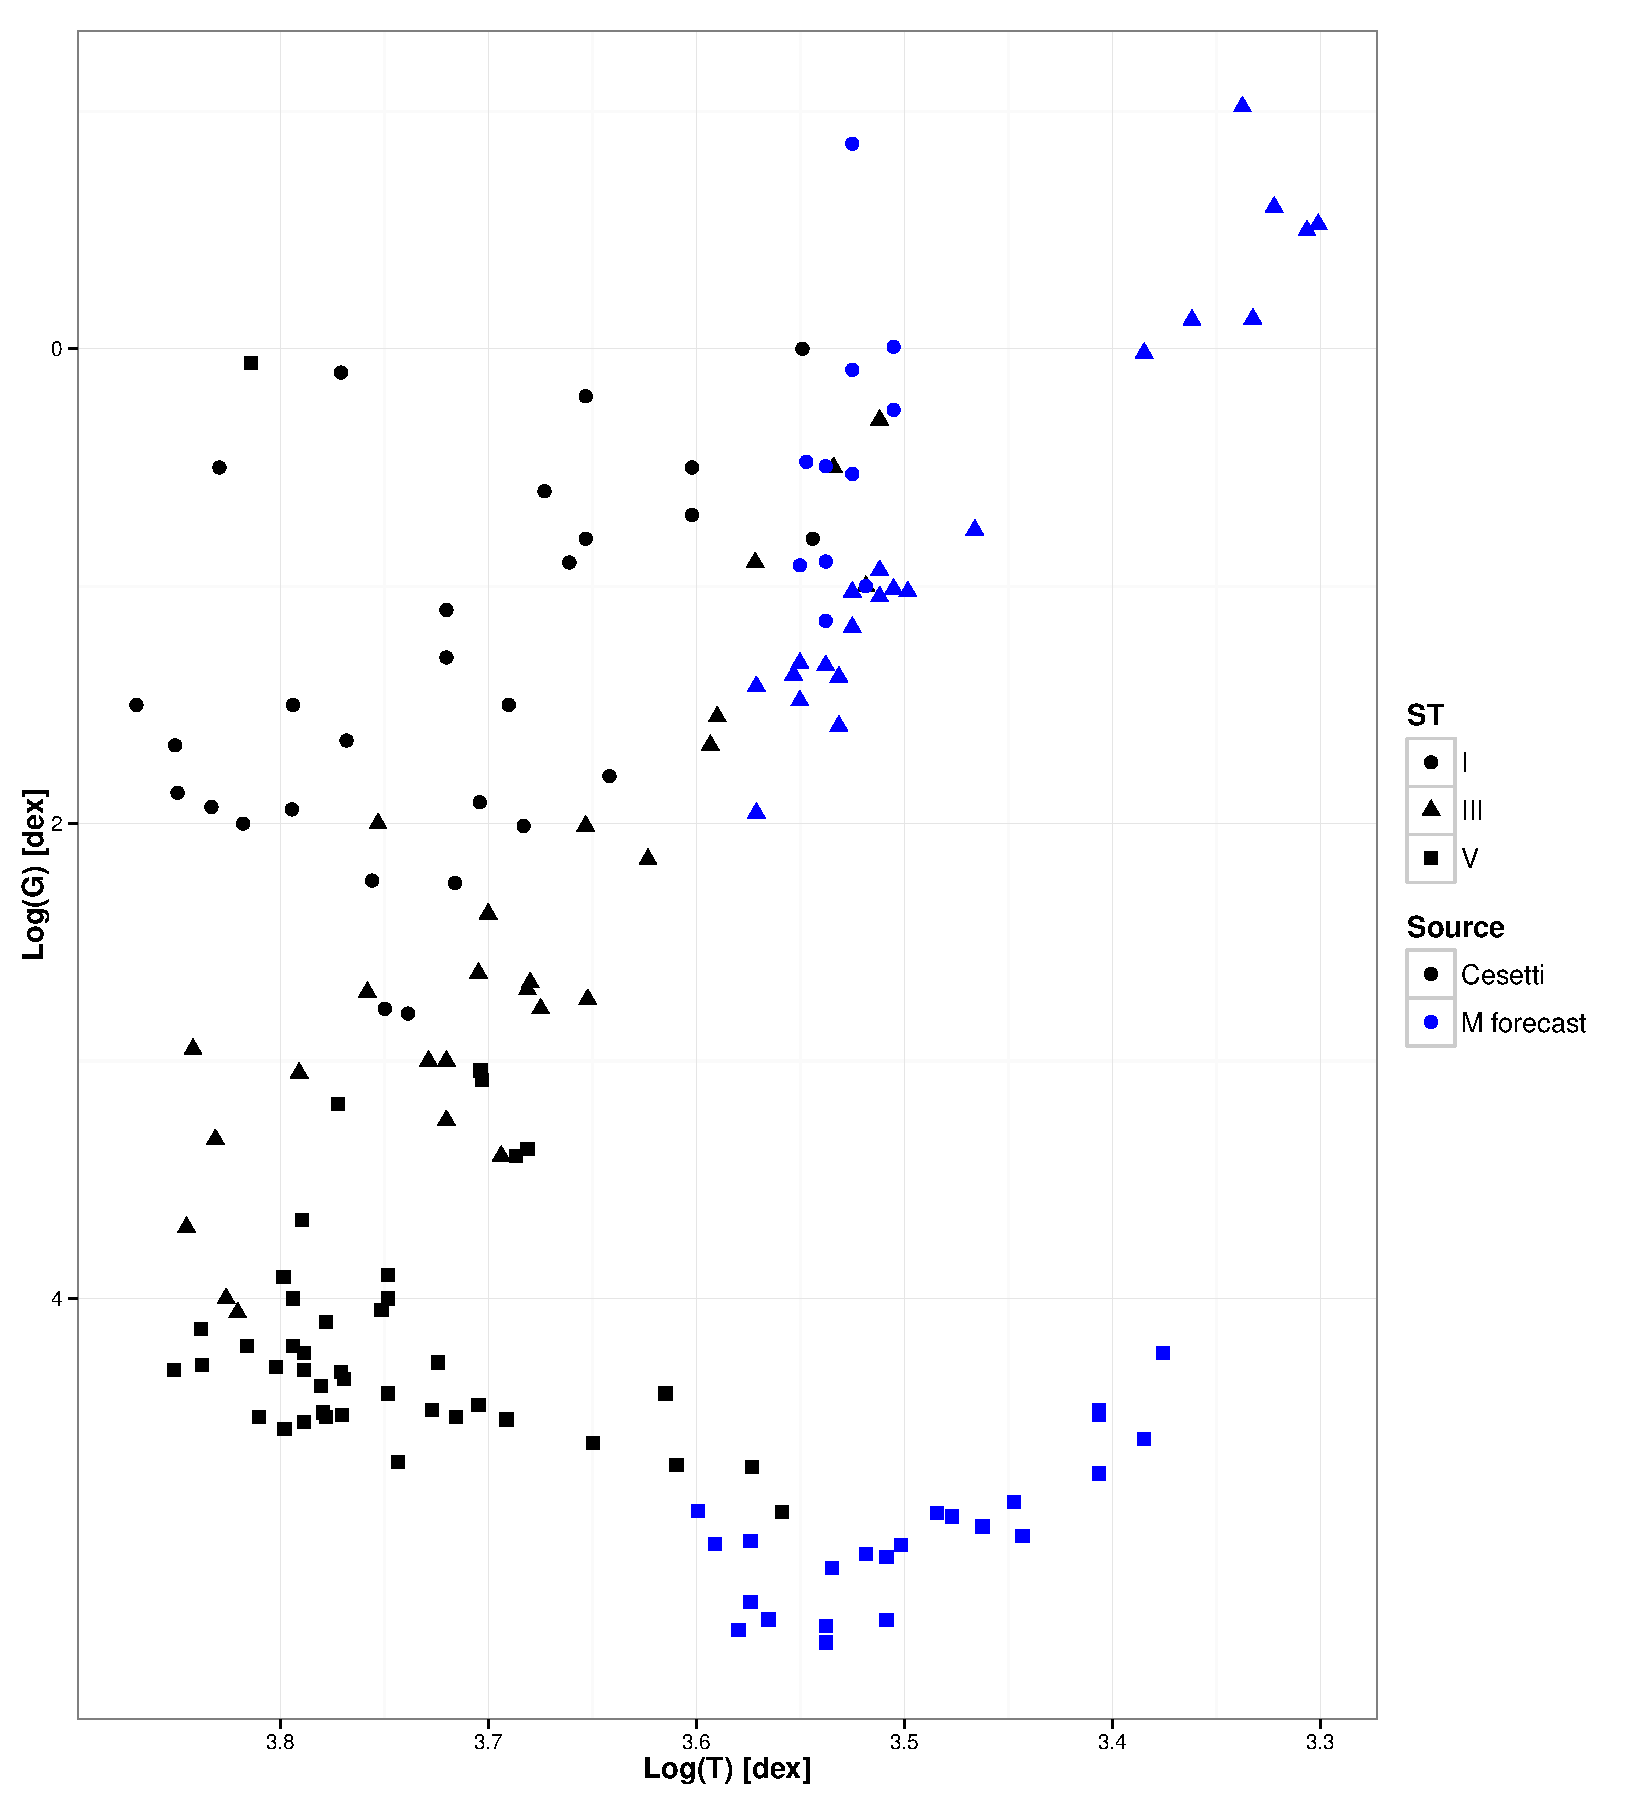
\includegraphics[width=12cm]{figs/irtf-logg-knn-oo.pdf}
 \caption{Relationship between $log(T_{eff}) $ in the x axis 
 and $log(g)$ in the y axis for KNN model based on the GA provided bandpass features with SNR=$\infty$}
 \label{fig:lt_lg_ga}
 \end{center}
\end{figure}

%And, for sure, it is possible to do it for estimations based on 
%parameters from nearest labeled BT-Settl spectra.
%In this particular case, it is possible to see how 
%considering the global spectrum is positive for stronger 
%physical parameters like $T_{eff}$ but the approach
%reduces drastically its likelihood when other softer 
%parameters are involved.
%
%\begin{figure}
% \begin{center}
% 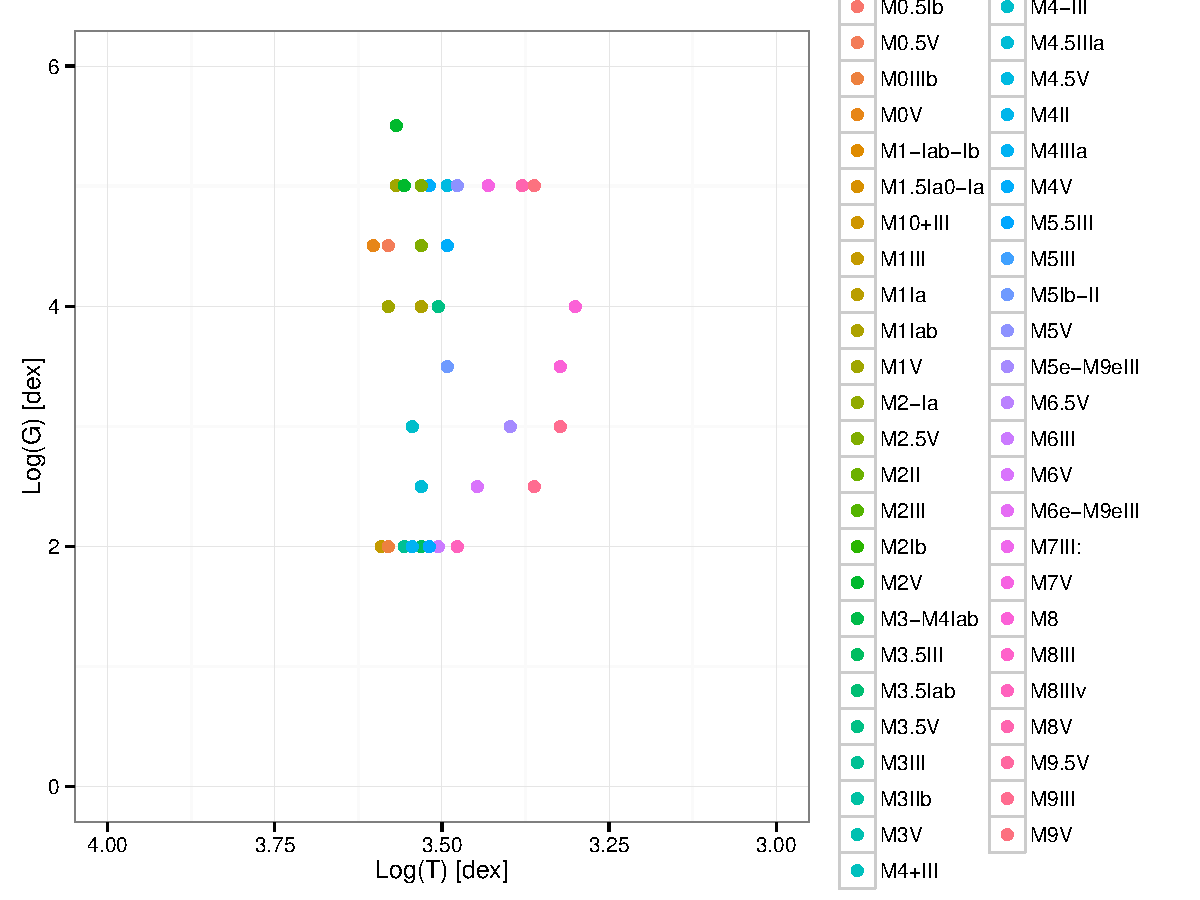
\includegraphics[width=12cm]{figs/LT_LG_chi2.pdf}
% \caption{Relationship between $log(T_{eff}) $ in the x axis 
% and $log(g)$ in the y axis for SNR=50 when 
% the nearest BT-Settl spectrum is used.}
% \label{fig:lt_lg_chi2}
% \end{center}
%\end{figure}
%
% Se debe realizar una intepretación, pero dependerá 
% 
% In Figure~\ref{fig:chi2_50_spt} and Figure~\ref{fig:ga_too50ga_spt} 
% relationships between $log(g)$ predicted by global espectrum estimation 
% and GA feature based estimation can be observed.
% 
% \begin {figure}
%  \centering
%  \begin{subfigure}{.85\textwidth}
%   \centering
%   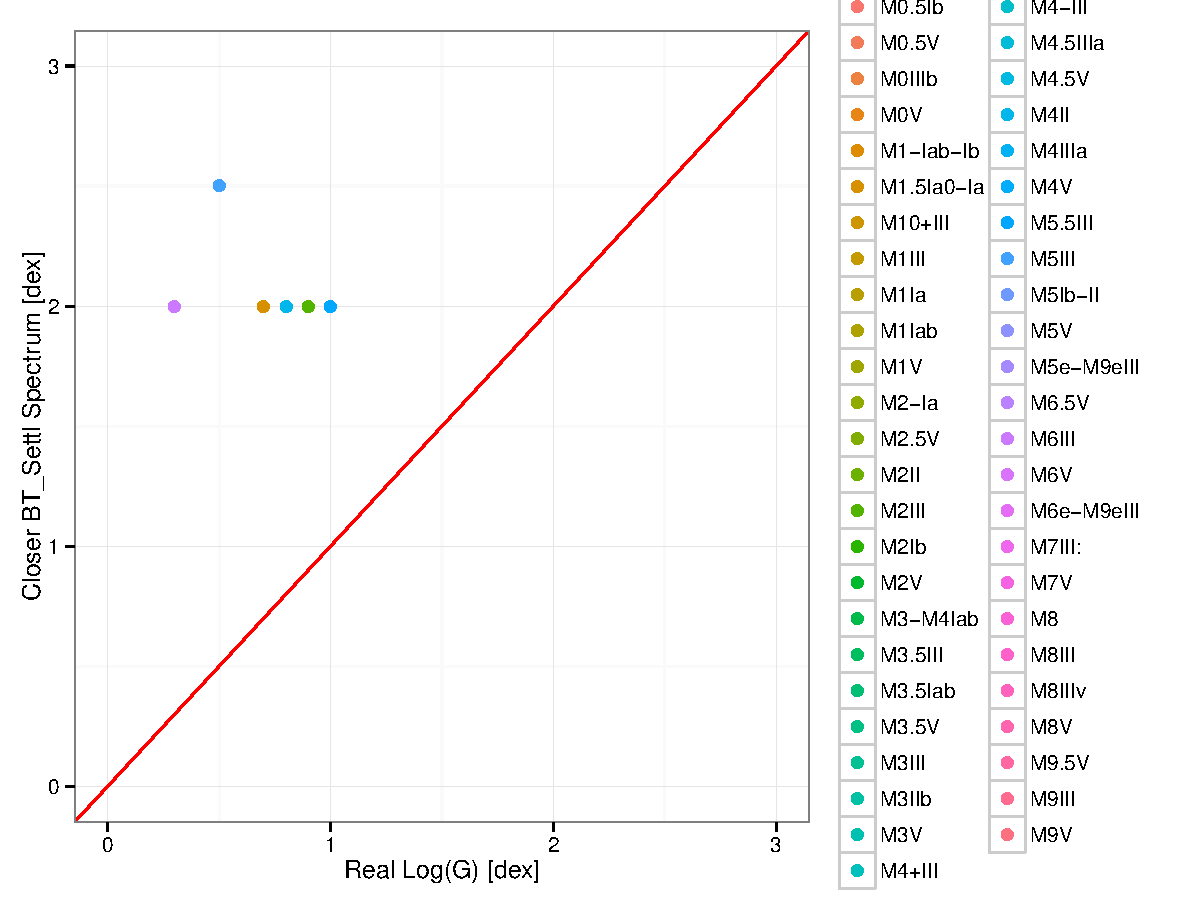
\includegraphics[width=12cm]{figs/G_chi2_50_cesetti.pdf}
%   \caption{Comparison between Gravity estimations from Spectral Subtype 
%  in x axis and the closest BT\_Settl spectra by $\chi^2$ at SNR=$50$ on y-axis}
%  \label{fig:chi2_50_spt}
%  \end{subfigure}
%   \begin{subfigure}{.85\textwidth}
%   \centering
%   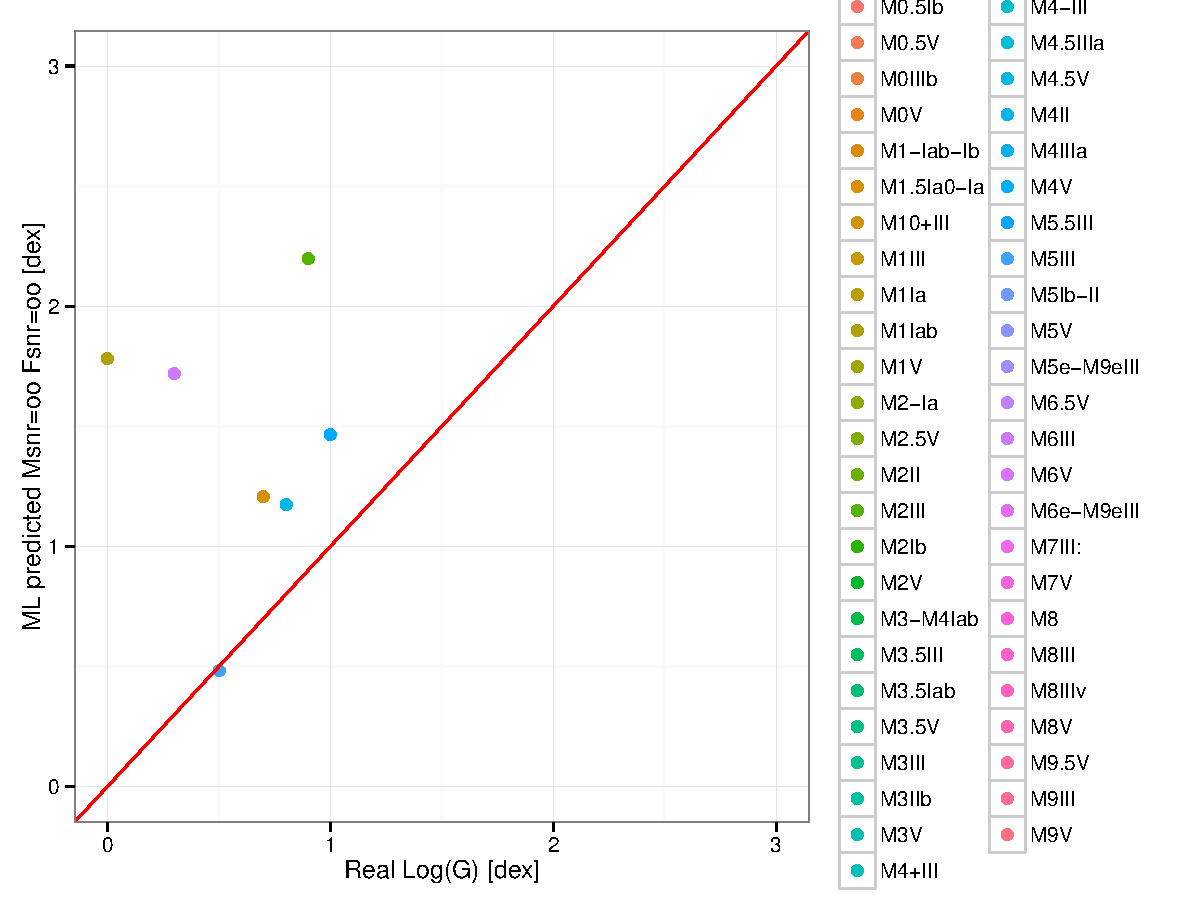
\includegraphics[width=12cm]{figs/G_gam_oo_cesetti.pdf}
%   \caption{Comparison between Gravity estimations from Spectral Subtype 
%  in x axis and the Support Vector Machines for Ga based features trained with BT\_Settl 
%  at SNR=$\infty$ and features for forecasting at SNR=$\infty$ on y-axis}
%  \label{fig:ga_too50ga_spt}
%  \end{subfigure}
%  \label {fig:comp02}
%  \caption{Performance comparison between the $chi^2$ based selection 
%           and the band oriented features to forecast Log(g)}
% \end {figure}
% %

% De nuevo las valoraciones deberían esperar a ver qué ponemos.

\subsection{Metallicity models} 

Finally, the same analysis is performed for the Metalicty parameter, 
again by considering Temperature as a fixed feature.
In Table~\ref{tab:models_M_rmse} 
we can see the analysis of performance of different classes of
models and cosidering a variety in features, even though just six IRTF stars 
where estimated by \cite{cesetti}, which strongly reduces the validation technique.

%
% Metalicidad teórica desde Cesseti para las IRTF
%
\ra{1.3}
\begin{table*}\centering
\begin{tabular}{@{}rrrcrrcrr@{}}\toprule
& \multicolumn{2}{c}{$SNR = 10$} & \phantom{ab}& \multicolumn{2}{c}{$SNR = 50$} &
\phantom{ab} & \multicolumn{2}{c}{$SNR = \infty$}\\
\cmidrule{2-3} \cmidrule{5-6} \cmidrule{8-9}
$Regression Models$ & $RMSE$ & $RMDSE$ && $RMSE$ & $RMDSE$     && $RMSE$       & $RMDSE$ \\ \midrule
$\chi^2 BTSettl$    &  0.76    & 0.22   && 0.36      & 0.18     && 0.36          & 0.18 \\
$ ICA+ ppr$         & \bf{0.24} & \bf{0.13} && \bf{0.31}  & 0.22 && 0.43       & 0.27 \\
$rf $               & \bf{0.33} & 0.25    && 0.73   & 0.41      && 0.61       & 0.36 \\
$gbm $              & \bf{0.27} & \bf{0.19} && 0.70  & 0.52      && 0.63      & 0.35 \\
$ svr $             & \bf{0.33} & 0.22       && 0.45 & 0.32       && 0.92      & 0.89 \\
$ nnet $            & \bf{0.37} & 0.30      && \bf{0.33} & 0.37    && 0.95    & 0.81 \\
$ knn $             & \bf{0.69}  & 0.55     && \bf{0.23}   & \bf{0.15} && \bf{0.21} & \bf{0.15} \\ 
$ mars+ bagging $   & \bf{0.36}  & \bf{0.16} && 0.49     & 0.41      && 0.83    & 0.85 \\
$Rule Regression $  & \bf{0.31} & \bf{0.17} && \bf{0.30} & 0.24  && 0.78 &  0.23 \\

\bottomrule
\end{tabular}
\caption {RMSE and RMDSE for the various regression models predicting $Met$ [dex].} 
\label{tab:models_M_rmse} 
% \end{center}
\end{table*}

 

% In Figure~\ref{fig:M_chi2_50_cesetti} and Figure~\ref{fig:M_GAM_1010_Cesetti} 
% relationships between metalicity predicted by global espectrum estimation 
% and GA feature based estimation against the real values
% provided by \cite{2013A&A...549A.129C} can be observed.

% \begin {figure}
%  \centering
%  \begin{subfigure}{.85\textwidth}
%   \centering
%   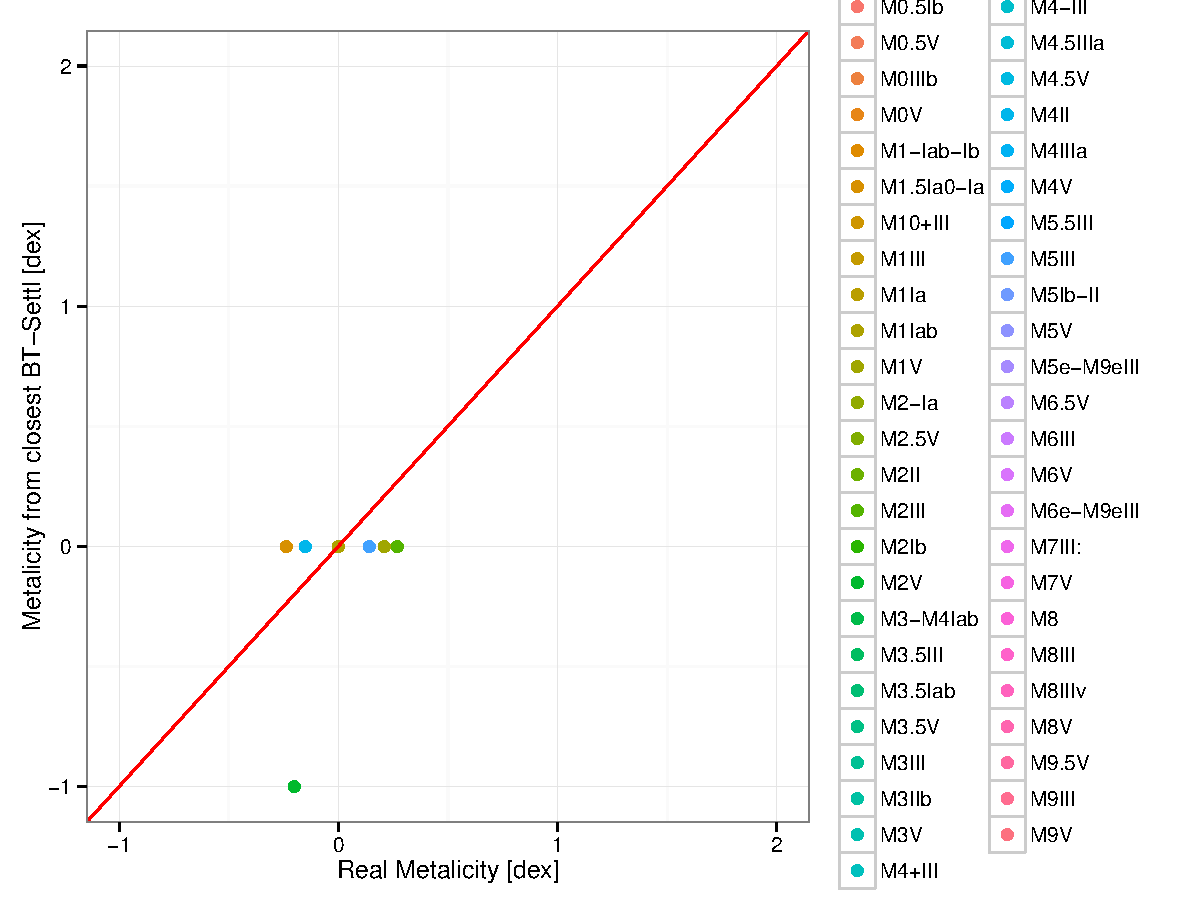
\includegraphics[width=12cm]{figs/M_Chi2_50_Cesetti.pdf}
%   \caption{Comparison between Metalicity estimations from Spectral Subtype 
%  in x axis and the closest BT\_Settl spectra by $\chi^2$ at SNR=$50$ on y-axis}
%  \label{M_chi2_50_cesetti}
%  \end{subfigure}
%   \begin{subfigure}{.85\textwidth}
%   \centering
%   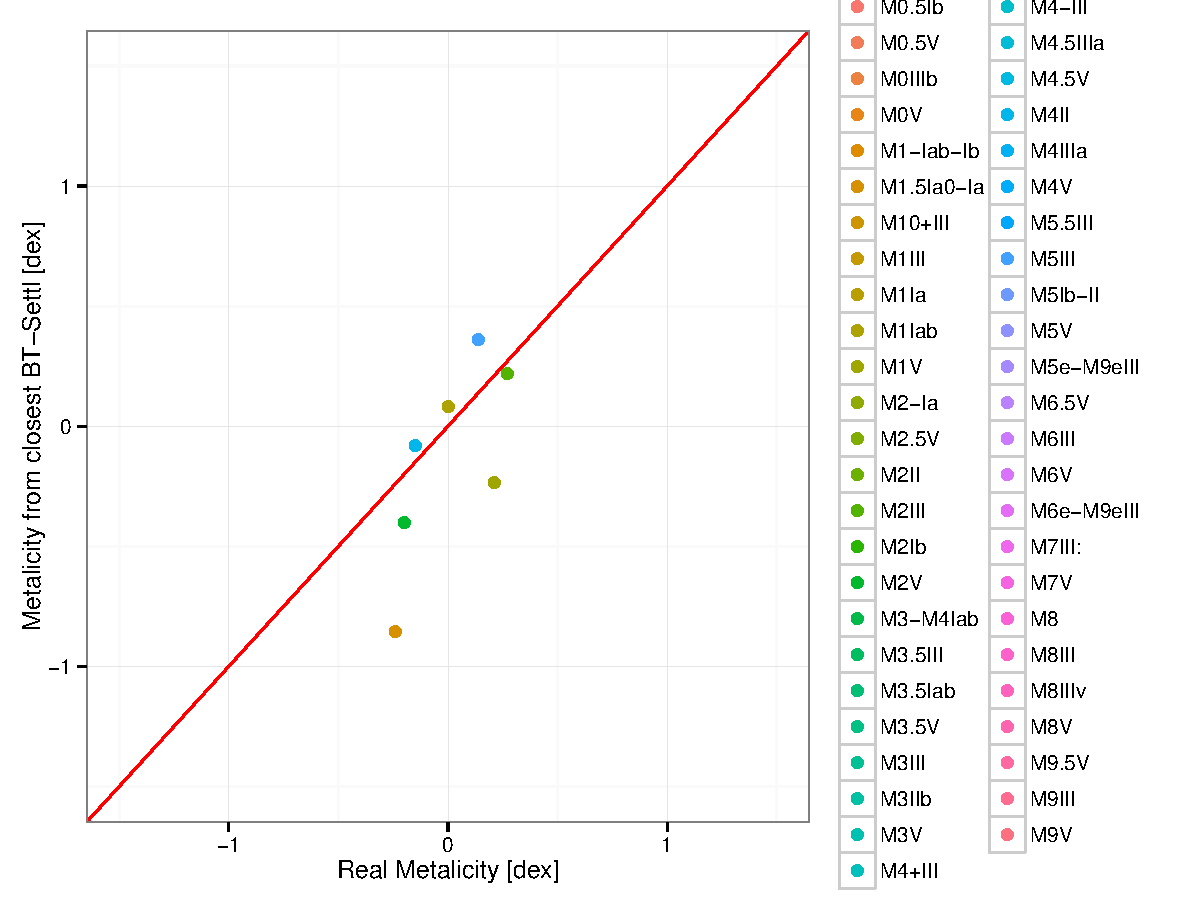
\includegraphics[width=12cm]{figs/M_GAM_1010_Cesetti.pdf}
%   \caption{Comparison between Metalicity estimations from Spectral Subtype 
%  in x axis and the Support Vector Machines for Ga based features trained with BT\_Settl 
%  at SNR=$\infty$ and features for forecasting at SNR=$\infty$ on y-axis}
%  \label{fig:M_GAM_1010_Cesetti}
%  \end{subfigure}
%  \label {fig:comp03}
%  \caption{Performance comparison between the $chi^2$ based selection 
%           and the band oriented features to forecast Log(g)}
% \end {figure}
%
   
   

% De nuevo, el análisis y discusión, función de lo que queramos dejar

